%%%%%%%%%%%%%%%%%%%%%%%%%%%%%%%%%%%%%%%%%%%%%%%%%%
%% Bachelor's & Master's Thesis Template        %%
%% Copyleft by Dawid Weiss & Marta Szachniuk    %%
%% Faculty of Computing and Telecommunication   %%
%% Poznan University of Technology, 2020        %%
%%%%%%%%%%%%%%%%%%%%%%%%%%%%%%%%%%%%%%%%%%%%%%%%%%


% Szkielet dla pracy licencjackiej pisanej w języku polskim.

\documentclass[polish,bachelor,a4paper,oneside]{ppfcmthesis}


\usepackage[utf8]{inputenc}
\usepackage[OT4]{fontenc}

%--------------------------------------
% Strona tytułowa
%--------------------------------------

% Autorzy pracy, jeśli jest ich więcej niż jeden
% wstaw między nimi separator \and
\author{%
   Mateusz Biernacki \album{140681} \and 
   Dominik Boła \album{136524} \and 
   Maciej Goral \album{132228} \and 
   Grzegorz Piątkowski \album{135868}}
\authortitle{}                                % Do not change.

\title{Aplikacja internetowa służąca do generowania planów lekcji dla szkół podstawowych oraz średnich}

% Your supervisor comes here.
\ppsupervisor{~dr~inż.~Izabela Janicka-Lipska} 

% Year of final submission (not graduation!)
\ppyear{2022}                                 


\begin{document}

% Front matter starts here
\frontmatter\pagestyle{empty}%
\maketitle\cleardoublepage%

%--------------------------------------
% Miejsce na kartę pracy dyplomowej
%--------------------------------------

\thispagestyle{empty}\vspace*{\fill}%
\begin{center}Tutaj będzie karta pracy dyplomowej;\\oryginał wstawiamy do wersji dla archiwum PP, w pozostałych kopiach wstawiamy ksero.\end{center}%
\vfill\cleardoublepage%

%--------------------------------------
% Spis treści
%--------------------------------------

\pagenumbering{Roman}\pagestyle{ppfcmthesis}%
\tableofcontents* 
\cleardoublepage % Zaczynamy od nieparzystej strony

%--------------------------------------
% Rozdziały
%--------------------------------------

%Najwygodniej jeśli każdy rozdział znajduje się w oddzielnym pliku
\mainmatter%

\chapter{Wstęp}
(Źródła?)Tematem podjętym w pracy jest aplikacja służąca do generowania planów zajęć. Główną motywacją do podjęcia takiego (tego?,"") tematu stanowią wady obecnie stosowanego przez większość szkół manualnego tworzenia planów zajęć. Ręczne tworzenie planu jest czasochłonne i wymaga dużego nakładu pracy. Dla osób odpowiedzialnych za ich przygotowanie (dalej zwanymi planistami) jest to zadanie monotonne, a także przytłaczające. Planiści, nawet ci z dużym doświadczeniem, nie są zdolni do utworzenia planu, który optymalnie wykorzystywałby godziny uczniów, nauczycieli, a także dostępność sali lekcyjnych. Skutkuje to znaczną liczbą niewykorzystanego czasu w środku dnia lekcyjnego.

Celem pracy jest zaprojektowanie aplikacji, dzięki której po podaniu niezbędnych danych, możliwe byłoby automatyczne wygenerowanie planu zajęć dla szkoły. Aplikacja ma umożliwić planiście dodawanie danych o przedmiotach, nauczycielach, salach i klasach. Na podstawie podanych danych planista ma mieć możliwość generacji rozkładu zajęć dla wszystkich klas w szkole. Aplikacja ma być przeznaczona dla szkół podstawowych oraz średnich. Ograniczenie to wynika z założenia niepodzielności klasy. W przypadku uczelni wyższych niejednolity podział na grupy znacząco zwiększa poziom skomplikowania rozwiązywanego problemu.

Praca ma następującą strukturę. Rozdział drugi poświecony jest podstawom teoretycznym. Rozdział trzeci zawiera analizę problemu i dostępnych rozwiązań. Rozdział czwarty to opis metodologii pracy. Rozdział piąty omawia część fronendową aplikacji. Rozdział szósty charakteryzuje backend aplikacji. Rozdział siódmy wyjaśnia działanie algorytmu generacji planu. Rozdział ośmy stanowią wnioski. Rozdział dziewiąty jest podumowaniem pracy. 

Implementacja aplikacji została wykonana przez cztery osoby.
Mateusz Biernacki wykonał ...
Dominik Boła wykonał ...
Maciej Goral wykonał ...
Grzegorz Piątkowski wykonał ...

Wstęp do pracy powinien zawierać następujące elementy:
\begin{itemize}
    \item krótkie uzasadnienie podjęcia tematu; 
    \item cel pracy (patrz niżej); 
    \item zakres (przedmiotowy, podmiotowy, czasowy) wyjaśniający, w jakim rozmiarze praca będzie realizowana; 
    \item ewentualne hipotezy, które autor zamierza sprawdzić lub udowodnić; 
    \item krótką charakterystykę źródeł, zwłaszcza literaturowych; 
    \item układ pracy (patrz niżej), czyli zwięzłą charakterystykę zawartości poszczególnych rozdziałów; 
    \item ewentualne uwagi dotyczące realizacji tematu pracy np.~trudności, które pojawiły się w trakcie 
    realizacji poszczególnych zadań, uwagi dotyczące wykorzystywanego sprzętu, współpraca z firmami zewnętrznymi. 
\end{itemize}

\noindent
\textbf{Wstęp do pracy musi się kończyć dwoma następującymi akapitami:}
\begin{quote}
Celem pracy jest opracowanie / wykonanie analizy / zaprojektowanie / ...........
\end{quote}
oraz:
\begin{quote}
Struktura pracy jest następująca. W rozdziale 2 przedstawiono przegląd literatury na temat ........ 
Rozdział 3 jest poświęcony ....... (kilka zdań). 
Rozdział 4 zawiera ..... (kilka zdań) ............ itd. 
Rozdział X stanowi podsumowanie pracy. 
\end{quote}

W przypadku prac inżynierskich zespołowych lub magisterskich 2-osobowych, po tych dwóch w/w akapitach 
musi w pracy znaleźć się akapit, w którym będzie opisany udział w pracy poszczególnych członków zespołu. Na przykład:

\begin{quote}
Jan Kowalski w ramach niniejszej pracy wykonał projekt tego i tego, opracował ......
Grzegorz Brzęczyszczykiewicz wykonał ......, itd. 
\end{quote}


% Co to jest NP - https://dbpedia.org/page/NP_(complexity)
% Co to jest problem NP-Trudny - https://www.baeldung.com/cs/p-np-np-complete-np-hard
% Ułozenie planu zajęć jako problem np-trudny - https://www.sciencedirect.com/science/article/pii/S1110016816000703#b0015


\chapter{Podstawy teoretyczne}
\section{Problem optymalizacyjny}
Problem optymalizacyjny~\cite{optimization_problem} jest to problem obliczeniowy, który polega na znalezieniu maksymalnej/minimalnej wartości pewnego parametru. Wartość takiego parametru zazwyczaj opisywana jest funkcją, dzięki której wartość parametru zależna jest od przeszukiwanych danych wejściowych. Jeśli poszukiwana jest jak najmniejsza wartość parametru, mówimy o problemie minimalizacyjnym i odpowiednio w przypadku poszukiwania największej wartości parametru, mówimy o problemie maksymalizacyjnym.

\section{Problem NP-trudny}
Problem NP-trudny~\cite{np_hard} jest problemem obliczeniowym, dla którego nie jest możliwym znalezienie rozwiązania w czasie wielomianowym przy wykorzystaniu niedeterministycznej maszyny Turinga, a sprawdzenie znalezionego rozwiązania jest co najmniej tak trudne jak każdego innego problemu z grupy NP. Problem optymalizacyjny jest jednym z problemów należących do grupy NP-trudnych.

\section{Heurystyka}
Heurystyka~\cite{heuristic} jest techniką rozwiązywania problemów w przypadku, gdy znalezienie dokładnego rozwiązania jest zbyt kosztowne. Metoda heurystyczna oferuje zmniejszenie kosztów rozwiązania problemu, jednak ceną takiego podejścia jest spadek dokładności rozwiązania czy nawet jego poprawności.  Przy wykorzystaniu metody heurystycznej otrzymanie optymalnego rozwiązania możliwe jest tylko w szczególnych przypadkach. Tego typu podejście wykorzystuje się również, w przypadku, gdy algorytm dokładny umożliwiający znalezienie rozwiązania optymalnego nie jest znany, w celu zawężenia pola badań.

\section{Algorytm ewolucyjny}
Algorytm ewolucyjny~\cite{evolution_algorithm} jest heurystycznym podejściem do rozwiązywania problemów, które nie mogą zostać rozwiązane w czasie wielomianowym, takie jak grupa problemów NP-trudnych, czy po prostu w celu zmniejszenia kosztów znalezienia rozwiązania problemu. Algorytmy ewolucyjne stosowane samodzielnie używane są zazwyczaj do rozwiązywania problemów optymalizacyjnych. Zastosowanie i działanie algorytmu ewolucyjnego jest bardzo proste do zrozumienia ze względu na to, że mamy do czynienia na co dzień z podobnym zjawiskiem w naturze czyli z selekcją naturalną. Przebieg działania algorytmu ewolucyjnego składa się z 4 głównych kroków.
	\begin{enumerate}
	\item \textbf{Inizjalizacja} -- W celu rozpoczęcia działania algorytmu, potrzebna jest pierwsza grupa rozwiązań (dalej nazywana populacją). Populacja zwierać będzie założoną liczbę możliwych rozwiązań (dalej nazywaną osobnikami). Zazwyczaj podczas inicjalizacji osobniki tworzone są w sposób losowy. Takie podejście jest wręcz zalecane, ponieważ umożliwia to przebadanie dużej różnorodności osobników, dzięki czemu finałowe rozwiązanie będzie lepsze.
	\item \textbf{Selekcja} -- Gdy pierwotna populacja jest gotowa, jej osobniki trzeba poddać ocenie. Funkcja oceny powinna składać się ze ściśle opisanych warunków opisujących środowisko, do którego osobniki muszą się przystosować. Im dokładniej środowisko zostanie opisane w funkcji oceny, tym lepsze będzie finalne rozwiązanie. Gdy funkcja jest poprawnie przygotowana, każdy z osobników musi zostać poddany ocenie, po której otrzymuje parametr oceny. Dzięki temu można wyróżnić rozwiązania lepsze od reszty. Z populacji zostaje wybrana założona liczba osobników o najwyższym parametrze oceny. Reszta osobników zostaje zabita.
	\item \textbf{Ewolucja} -- Ewolucja składa się z dwóch kroków: krzyżowania oraz mutacji. 
	\begin{enumerate}
		\item Krzyżowanie -- po otrzymaniu wybranych osobników z selekcji, użyte są one do stworzenia nowego pokolenia dla algorytmu, stając się osobnikami-rodzicami. Wykorzystując charakterystyki osobników-rodziców, utworzona zostaje populacja osobników-dzieci poprzez wymieszanie ze sobą charakterystyk osobników-rodziców. Po utworzeniu nowego pokolenia osobników-dzieci, osobniki-rodzice zostają zabite.
		\item Mutacja -- jest to prawdopodobnie najważniejszy krok ewolucji. Bez niego cała populacja bardzo szybko utknęłaby w miejscu, nie oferując żadnego sensownego rozwiązania. W tym kroku charakterystyka każdego osobnika-dziecka z nowego pokolenia poddana jest małym losowym zmianom w celu zróżnicowania ich od osobników-rodziców. Na końcu tego kroku osobniki-dzieci stają się nowym pokoleniem osobników w populacji, która może ponownie zostać poddana selekcji.
	\end{enumerate}
	\item \textbf{Finalizacja} -- Ostatecznie działanie algorytmu musi dobiec końca. W tym kroku z populacji zostaje wybrany osobnik z najwyższym parametrem oceny i zwrócony jako rozwiązanie. Są dwie możliwości, w których zakończenie działania algorytmu może zostać wywołane. Gdy osiągnie on maksymalny czas działania (np. założona maksymalna liczba pokoleń) lub gdy osiągnięty zostanie poszukiwany pułap parametru oceny.
	\end{enumerate}	



\chapter{Analiza i porównanie możliwych rozwiązań}
\section{Analiza problemu}
Podstawowym problemem w automatycznym tworzeniu planu zajęć jest dobór warunków wykorzystywanych przy generacji. Warunki te można podzielić na niezbędne do utworzenia poprawnego planu oraz warunki dodatkowe, których spełnienie zwiększa użyteczność planu z punktu widzenia planisty. 

Wśród warunków niezbędnych należy wyróżnić warunek braku konfliktów. Konflikt ma miejsce, gdy występuje jedna z następujących sytuacji:
\begin{itemize}
    \item w jednej godzinie lekcyjnej, jednej klasie został przyporządkowany więcej niż jeden przedmiot,
    \item w jednej godzinie lekcyjnej, jednemu nauczycielowi została przyporządkowana więcej niż jedna klasa,
    \item w jednej godzinie lekcyjnej, jednej sali została przyporządkowana więcej niż jedna klasa.
\end{itemize}
W przypadku szkół podstawowych oraz średnich do warunków niezbędnych należy również zaliczyć brak niewykorzystanych godzin w środku dnia lekcyjnego uczniów. Dodatkowo niektóre zajęcia, takie jak wychowanie fizyczne, mogą być przeprowadzone tylko w specjalnie przeznaczonych do tego salach.

Warunki dodatkowe mogą różnić się w zależności od czynników, które należy wziąć pod uwagę przy pod uwagę przy generacji plany wynikających ze specyfikacji szkoły oraz wymagań personelu dydaktycznego. Do tych czynników można zaliczyć:
\begin{itemize}
    \item ograniczenia dostępności nauczycieli, wynikające z pracy w innych placówkach oświatowych lub innych powodów,
    \item ograniczenia wynikające z odległości między salami,
    \item obecność zajęć nieobowiązkowych, które muszą w danym dniu lekcyjnym być skrajnie pierwsze lub ostatnie,
    \item  konieczność minimalizacji niewykorzystanych godzin w środku dnia lekcyjnego dla uczniów,
    \item konieczność grupowania zajęć w przypadku kilku godzin lekcyjnych tego samego przedmiotu jednego dnia -- w takim przypadku zajęcia te powinny następować bezpośrednio po sobie oraz w tej samej sali,
    \item konieczność równomiernego rozłożenie przedmiotów w trakcie tygodnia lekcyjnego.
\end{itemize}
\section{Aktualnie dostępne rozwiązania}
\subsection{aSc TimeTables}
aSc TimeTables~\cite{asc} to aplikacja desktopowa wspomagająca przygotowywanie planów zajęć. Narzędzie umożliwia generowanie planów na podstawie zdefiniowanych wymagań, wprowadzenie do nich ręcznych poprawek oraz wyszukiwanie konfliktów we wprowadzonych zmianach. aSc TimeTables jest najbardziej rozbudowanym rozwiązaniem tego typu dostępnym na rynku, pozwalającym na tworzenie planów zajęć dla szkół i uczelni. Do dodatkowych funkcji programu należy możliwość importu danych z pliku, zdolność mapowania szkoły oraz udostępnienia planów uczniom i nauczycielom za pomocą aplikacji mobilnej. Z wszechstronnością i bogactwem funkcji wiąże się wysoki poziom umiejętności potrzebny do poprawnego wykorzystania aplikacji. Do pozostałych wad programu należy brak regularnych aktualizacji, podatność na błędy w generacji planu, wysoka cena oraz dostępność ograniczona do systemu Windows.
\subsection{Prime Timetable}
Prime Timetables~\cite{prime} to aplikacja internetowa przeznaczona dla organizacji edukacyjnych umożliwiająca zarówno ręczne jak i automatyczne układanie planów lekcji. Prime Timetables pozwala na wspólne tworzenie planów przez kilku użytkowników oraz udostępnianie gotowych planów dla uczniów i nauczycieli posiadających konta w serwisie. Aplikacja posiada rozbudowany zestaw narzędzi umożliwiających określanie ograniczeń związanych z automatyczną generacją planu. Główną wadą rozwiązania jest wysoka opłata miesięczna, której wysokość dodatkowo zależy od liczby nauczycieli w szkole. 
\subsection{SuperSaas}
SuperSaas~\cite{saas} to program do zarządzania szkołami i innymi instytucjami, którego głównym atutem jest wbudowany system rezerwacji. Przy pomocy konta WordPress użytkownicy aplikacji mogą umawiać terminy wizyt, a także dokonywać za nie płatności. SuperSaas cechuje niska cena oraz dostępność z poziomu przeglądarki. Duża część funkcjonalności aplikacji nie jest przeznaczona dla szkół. Pomimo możliwości wspomagania ręcznego układania planów zajęć, program nie pozwala na automatyczną ich generację, ani nawet wykrywanie konfliktów. 
\section{Możliwe podejścia}
Możliwe rozwiązania można podzielić w zależności od kilku aspektów. Pierwszym z nich jest wybór rodzaju aplikacji -- desktopowej, mobilnej lub internetowej. Ze względu na fakt, że korzystanie z aplikacji wymagać ma wprowadzania dużej ilości danych, można założyć, że z punktu widzenia użytkownika najkorzystniejsze będzie użycie w tym celu fizycznej klawiatury. Powoduje to odrzucenie wyboru aplikacji mobilnej. Zaletami  wyboru aplikacji desktopowej jest możliwość korzystania z niej bez dostępu do Internetu oraz bezpieczeństwo związane z lokalnym przechowywaniem danych. Pomimo tych korzyści rozwiązanie to nie oferuje zalet związanych z wyborem aplikacji internetowej -- dostępu z dowolnego urządzenia wyposażonego w kompatybilną przeglądarkę, braku wymagań systemowych związanych z obliczeniami i przechowywaniem danych oraz braku konieczności aktualizowania aplikacji przez użytkownika. Te czynniki jednoznacznie przesądzają o wykorzystaniu w projekcie aplikacji internetowej.

Drugim aspektem, który należy rozpatrzyć jest poziom złożoności aplikacji, związany głównie z wyborem możliwych do wprowadzenia przez planistę warunków wykorzystywanych przy generacji planu. Większa liczba warunków może wiązać się z lepszą jakością planu, ale także dłuższym czasem jego generacji. Należy również rozpatrzyć stosunek nakładu pracy przeznaczonej na implementację warunku w stosunku do potencjalnego zysku dla użytkowników. Każdy dodatkowy warunek spowodowałby zmniejszenie przejrzystości interfejsu graficznego, szczególnie dla użytkowników, dla których byłby on zbędny. Biorąc pod uwagę te czynniki w projekcie wykorzystane zostaną jedynie te warunki, których obecność jest niezbędna do poprawnej generacji planu.

Ostatnim ważnym do rozpatrzenia aspektem jest wybór użytkowników, którzy będą posiadać konta w systemie. Pierwszym z nich jest planista -- osoba odpowiedzialna za układanie planów. W rozwiązaniu, w których planiści nie posiadają kont, wprowadzone informacje nie byłyby przechowywane w bazie w danych, co oznacza ich utratę przypadku zakończenia sesji. Konieczność posiadania przez planistę konta eliminuje ten problem i dodatkowo utrudnia ataki na stronę. Pozostali potencjalni użytkownicy to nauczyciele oraz uczniowie. W projekcie zakładamy możliwość podania przez nauczyciela swojej dyspozycyjności. Ze względu na konieczność podania przez planistów adresu e-mail każdego dodanego nauczyciela, jest to możliwe poprzez unikatowy link wysłany w wiadomości, bez obowiązku zakładania konta. Dla uczniów, ze względu na brak bezpośredniego wpływu na plan zajęć, również nie zakłada się możliwości stworzenia konta. 
\section{Wymagania funkcjonalne i niefunkcjonalne}
Wymagania funkcjonalne:
\begin{itemize}
    \item możliwość rejestracji w aplikacji,
    \item możliwość logowania w aplikacji,
    \item możliwość dodania danych przedmiotów, nauczycieli, sal i klas,
    \item możliwość edycji danych przedmiotów, nauczycieli, sal i klas,
    \item możliwość usunięcia danych przedmiotów, nauczycieli, sal i klas,
    \item możliwość generacji planu na podstawie podanych danych,
     \item możliwość wyświetlania wygenerowanych planów z podziałem na plany dla klas, nauczycieli i sale,
    \item możliwość przesłania do nauczycieli ankiet dyspozycyjności,
    \item możliwość wypełnienia ankiety dyspozycyjności przez nauczyciela.
\end{itemize}
Wymagania niefunkcjonalne:
\begin{itemize}
    \item responsywność na urządzeniach mobilnych,
    \item uwierzytelnianie oparte o tokeny JWT,
    \item możliwość przerwania dodawania danych bez utraty postępu,
    \item kompatybilność z przeglądarkami Chrome, Firefox, Opera oraz Edge,
    \item formularze dodawania danych proste i intuicyjne w obsłudze,
    \item szyfrowanie danych w bazie danych.
\end{itemize}
\section{Przypadki użycia}
Na rysunku~\ref{rys:vuex} przedstawiono diagram przypadków użycia.
\begin{figure}[!ht]
\centering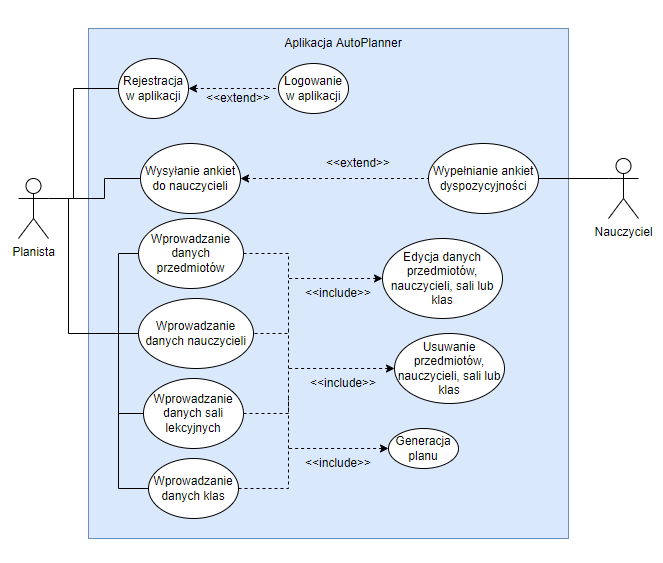
\includegraphics[width=\textwidth]{figures/DiagramPU}
\caption{Diagram przypadków użycia}\label{rys:pu}
\end{figure}


\noindent
\textbf{Przypadek użycia:} Rejestracja w aplikacji\\
\textbf{Aktor główny:} Planista\\
\textbf{Scenariusz główny:}
\begin{enumerate}
	\item Planista wpisuje adres e-mail.
	\item Aplikacja nie zgłasza problemu ze składnią adresu e-mail.
	\item Planista wpisuje nazwę użytkownika oraz hasło.
	\item Planista zatwierdza wprowadzone dane.
	\item Aplikacja akceptuje wprowadzone dane.
	\item Aplikacja tworzy nowe konto użytkownika.
\end{enumerate}
\textbf{Rozszerzenia:}
	\begin{enumerate}
         \item[2.A] Aplikacja zgłasza problem ze składnią adresu e-mail.
         \begin{enumerate}
         	\item[2.A.1] Planista poprawia składnię adresu e-mail.
         \end{enumerate}
         \item[5.A] Aplikacja zgłasza problem  dotyczący wymagań hasła.
         \begin{enumerate}
         	\item[5.A.1] Planista wpisuje hasło, które spełnia wymagania.
         \end{enumerate}
         \item[5.B] Aplikacja zgłasza, że na wpisany adres e-mail jest już założone konto.
         \begin{enumerate}
         	\item[5.B.1] Planista wpisuje nowy adres e-mail.
         \end{enumerate}
	\end{enumerate}
	
\noindent
\textbf{Przypadek użycia:} Logowanie w aplikacji\\
\textbf{Aktor główny:} Planista\\
\textbf{Scenariusz główny:}
\begin{enumerate}
	\item Planista wpisuje adres e-mail.
	\item Planista wpisuje hasło.
	\item Planista zatwierdza wprowadzone dane.
	\item Aplikacja akceptuje wprowadzone dane.
	\item Aplikacja przechodzi do widoku użytkownika zalogowanego.
\end{enumerate}
\textbf{Rozszerzenia:}
	\begin{enumerate}
         \item[4.A] Aplikacja zgłasza, że wprowadzone hasło jest nieprawidłowe.
         \begin{enumerate}
         	\item[4.A.1] Planista ponownie wpisuje hasło.
         \end{enumerate}
         \item[4.B] Aplikacja zgłasza, że użytkownik o podanym adresie e-mail nie istnieje.
         \begin{enumerate}
         	\item[4.B.1] Planista ponownie wpisuje adres e-mail.
         \end{enumerate}
	\end{enumerate}
	
\noindent
\textbf{Przypadek użycia:} Wprowadzanie danych przedmiotów\\
\textbf{Aktor główny:} Planista\\
\textbf{Scenariusz główny:}
\begin{enumerate}
	\item Planista wpisuje nazwę przedmiotu.
	\item Planista zatwierdza wprowadzone dane.
	\item Aplikacja akceptuje wprowadzone dane.
	\item Aplikacja dodaje przedmiot do listy z lewej strony ekranu.
\end{enumerate}
\textbf{Rozszerzenia:}
	\begin{enumerate}
         \item[3.A] Aplikacja zgłasza, że przedmiot o danej nazwie został już wcześniej wprowadzony.
         \begin{enumerate}
         	\item[3.A.1] Planista wpisuje nową nazwę przedmiotu.
         \end{enumerate}
         \item[3.B] Aplikacja zgłasza, że nazwa przedmiotu zawiera niedozwolone znaki.
         \begin{enumerate}
         	\item[3.B.1] Planista wpisuje nową nazwę przedmiotu.
         \end{enumerate}
	\end{enumerate}
	
\noindent
\textbf{Przypadek użycia:} Wprowadzanie danych nauczycieli\\
\textbf{Aktor główny:} Planista\\
\textbf{Scenariusz główny:}
\begin{enumerate}
	\item Planista wpisuje imię i nazwisko nauczyciela.
	\item Planista wpisuje adres e-mail nauczyciela.
	\item Aplikacja nie zgłasza problemu ze składnią adresu e-mail.
	\item Planista wybiera z listy wprowadzony przez nauczyciela przedmiot.
	\item Aplikacja akceptuje wprowadzone dane.
	\item Aplikacja dodaje nauczyciela do listy z lewej strony ekranu.
\end{enumerate}
\textbf{Rozszerzenia:}
	\begin{enumerate}
         \item[3.A] Aplikacja zgłasza problem ze składnią adresu e-mail.
         \begin{enumerate}
         	\item[3.A.1] Planista poprawia składnię adresu e-mail.
         \end{enumerate}
         \item[4.A] Planista dodaje kolejne przedmioty prowadzone przez nauczyciela.
         \item[5.A] Aplikacja zgłasza, że nauczyciel o danym adresie e-mail został już wcześniej wprowadzony.
         \begin{enumerate}
         	\item[5.A.1] Planista wpisuje nowy adres e-mail.
         \end{enumerate}
         \item[5.B] Aplikacja zgłasza, że imię lub nazwisko nauczyciela zawiera niedozwolone znaki.
         \begin{enumerate}
         	\item[5.B.1] Planista wpisuje nowe imię i nazwisko nauczyciela.
         \end{enumerate}
	\end{enumerate}

\noindent
\textbf{Przypadek użycia:} Wprowadzanie danych sal lekcyjnych\\
\textbf{Aktor główny:} Planista\\
\textbf{Scenariusz główny:}
\begin{enumerate}
	\item Planista wpisuje nazwę sali.
	\item Planista nie dodaje preferowanych przedmiotów.
	\item Planista zatwierdza wprowadzone dane.
	\item Aplikacja akceptuje wprowadzone dane.
	\item Aplikacja dodaje salę do listy z lewej strony ekranu.
\end{enumerate}
\textbf{Rozszerzenia:}
	\begin{enumerate}
         \item[2.A] Planista dodaje jeden lub więcej preferowany przedmiot.
         \item[4.A] Aplikacja zgłasza, że sala o danej nazwie została już wcześniej wprowadzona.
         \begin{enumerate}
         	\item[4.A.1] Planista wpisuje nową nazwę sali.
         \end{enumerate}
         \item[4.B] Aplikacja zgłasza, że nazwa sali zawiera niedozwolone znaki.
         \begin{enumerate}
         	\item[4.B.1] Planista wpisuje nową nazwę sali.
         \end{enumerate}
	\end{enumerate}
	
\noindent
\textbf{Przypadek użycia:} Wprowadzanie danych klas\\
\textbf{Aktor główny:} Planista\\
\textbf{Scenariusz główny:}
\begin{enumerate}
	\item Planista wpisuje nazwę klasy.
	\item Planista wybiera z listy kolejne przedmioty.
	\item Planista wpisuje tygodniowe liczby godzin dla każdego przedmiotu.
	\item Planista nie wybiera prowadzącego dany przedmiot.
	\item Planista zatwierdza wprowadzone dane.
	\item Aplikacja akceptuje wprowadzone dane.
	\item Aplikacja dodaje klasę do listy z lewej strony ekranu.
\end{enumerate}
\textbf{Rozszerzenia:}
	\begin{enumerate}
         \item[4.A] Planista wybiera z listy prowadzącego przedmiot.
         \item[6.A] Aplikacja zgłasza, że klasa o danej nazwie została już wcześniej wprowadzona.
         \begin{enumerate}
         	\item[6.A.1] Planista wpisuje nową nazwę klasy.
         \end{enumerate}
         \item[6.B] Aplikacja zgłasza, że nazwa klasy zawiera niedozwolone znaki.
         \begin{enumerate}
         	\item[6.B.1] Planista wpisuje nową nazwę klasy.
         \end{enumerate}
         \item[6.C] Aplikacja zgłasza, że wprowadzona liczba godzin ma nieprawidłowy format.
         \begin{enumerate}
         	\item[6.C.1] Planista wpisuje nową liczbę godzin.
         \end{enumerate}
	\end{enumerate}
	
\noindent
\textbf{Przypadek użycia:} Edycja danych przedmiotów, nauczycieli, sal lub klas\\
\textbf{Aktor główny:} Planista\\
\textbf{Scenariusz główny:}
\begin{enumerate}
	\item Planista wybiera przedmiot, nauczyciela, salę lub klasę, których dane chce edytować.
	\item Aplikacja przechodzi do ekranu edycji z aktualnymi danymi wybranego przedmiotu, nauczyciela, sali lub klasy.
	\item Planista edytuje dane.
	\item Planista zatwierdza edycję danych.
	\item Aplikacja akceptuje edycję danych.
	\item Aplikacja powraca do ekranu dodawania przedmiotu, nauczyciela, sali lub klasy.
\end{enumerate}
\textbf{Rozszerzenia:}
	\begin{enumerate}
         \item[5.A] Aplikacja zgłasza, że nowe dane są nieprawidłowe, w ten sam sposób jak miało to miejsce w przypadku ich dodawania.
         \begin{enumerate}
         	\item[5.A.1] Planista poprawia wpisane dane.
         \end{enumerate}
	\end{enumerate}
	
\noindent
\textbf{Przypadek użycia:} Usuwanie przedmiotów, nauczycieli, sal lub klas\\
\textbf{Aktor główny:} Planista\\
\textbf{Scenariusz główny:}
\begin{enumerate}
	\item Planista wybiera przedmiot, nauczyciela, salę lub klasę, których dane chce edytować.
	\item Aplikacja przechodzi do ekranu edycji z aktualnymi danymi wybranego przedmiotu, nauczyciela, sali lub klasy.
	\item Planista wybiera opcję usuń przedmiot, nauczyciela, salę lub klasę.
	\item Aplikacja usuwa przedmiot, nauczyciela, salę lub klasę z listy z lewej strony ekranu.
\end{enumerate}

\noindent
\textbf{Przypadek użycia:} Wysyłanie ankiet do nauczycieli\\
\textbf{Aktor główny:} Planista\\
\textbf{Scenariusz główny:}
\begin{enumerate}
	\item Planista wybiera opcję 'wyślij ankiety dyspozycyjności' na ekranie dodawania nauczycieli.
	\item Aplikacja wysyła wiadomości e-mail z ankietami dyspozycyjności na adresy e-mail wszystkich do tej pory dodanych nauczycieli.
	\item Aplikacja wyświetla informację, że ankiety zostały wysłane.
\end{enumerate}

\noindent
\textbf{Przypadek użycia:} Wypełnienie ankiety dyspozycyjności\\
\textbf{Aktor główny:} Nauczyciel\\
\textbf{Scenariusz główny:}
\begin{enumerate}
	\item Nauczyciel poprzez link w wiadomości e-mail przechodzi do ekranu wypełniania ankiety.
	\item Nauczyciel zaznacza w siatce godzin swoją dyspozycyjność.
	\item Nauczyciel zatwierdza wprowadzone dane.
	\item Aplikacja zapisuje dane w celu wykorzystania przy generacji planu.
\end{enumerate}

\noindent
\textbf{Przypadek użycia:} Generacja planu\\
\textbf{Aktor główny:} Planista\\
\textbf{Scenariusz główny:}
\begin{enumerate}
	\item Planista wybiera opcję 'generuj plan'.
	\item Aplikacja rozpoczyna generację planu i przechodzi do ekranu oczekiwania.
	\item Aplikacja kończy generację planu i przechodzi do ekranu szkoły.
	\item Planista przegląda wygenerowane plany z podziałem na plany klas, nauczycieli i sal lekcyjnych.
\end{enumerate}

\chapter{Metodyka pracy oraz przygotowanie infrastruktury informatycznej}

\section{Wstęp}
Projekt powstawał w metodyce DevOps. Takie podejście pozwoliło na szybsze dostarczenie finalnego produktu. Wysoki poziom kooperacji wynikający z metodki DevOps pozwolił na zmniejszenie kosztów dostarczenia produktu oraz znaczne zwiększenie jego spójności. Potrzebna jest jednak mocno rozwinięta infrastruktura informatyczna służąca podtrzymaniu DevOps lifecycle.

\section{Pojęcia}
	\subsection{DevOps}
	DevOps~\cite{devops} to zestaw praktyk, narzędzi i filozofii kulturowej, które automatyzują i integrują procesy pomiędzy zespołami programistów oraz IT. Kładzie nacisk na wzmocnienie pozycji zespołu, komunikację i współpracę między zespołami oraz automatyzację technologii.
	Ruch DevOps rozpoczął się około 2007 roku, kiedy społeczności programistów i operatorów IT wyraziły zaniepokojenie tradycyjnym modelem rozwoju oprogramowania, w którym programiści piszący kod pracowali oddzielnie od operatorów, którzy wdrażali i wspierali kod. Termin DevOps, będący połączeniem słów \textit{development} i \textit{operations}, odzwierciedla proces integracji tych dyscyplin w jeden, ciągły proces.
	\subsection{Continous Integration}
	\textit{Continous Integration and Continous Delivery} (CI/CD)~\cite{ci} to metoda częstego dostarczania aplikacji do klientów poprzez wprowadzenie automatyzacji do etapów tworzenia aplikacji. Główne pojęcia przypisane do CI/CD to ciągła integracja, ciągłe dostarczanie i ciągłe wdrażanie. CI/CD jest rozwiązaniem problemów, jakie integracja nowego kodu może powodować dla zespołów programistycznych i operacyjnych.
	W szczególności, CI/CD wprowadza ciągłą automatyzację i ciągłe monitorowanie w całym cyklu życia aplikacji, od fazy integracji i testowania po dostarczanie i wdrażanie. Łącznie, te połączone praktyki są często określane jako CI/CD i są wspierane przez zespoły programistów i operatorów pracujących razem zpodejściem DevOps lub SRE (\textit{site reliability engineering}).
	\subsection{Kontrola wersji}
	Kontrola wersji~\cite{version_control}, znana również jako kontrola źródła, jest praktyką śledzenia i zarządzania zmianami w kodzie oprogramowania. Systemy kontroli wersji to narzędzia programowe, które pomagają zespołom programistów zarządzać zmianami w kodzie źródłowym w czasie.


\section{Narzędzia i technologie}
	\subsection{Amazon Web Services}
	\textit{Amazon Web Services} (AWS)~\cite{aws} jest spółką zależną firmy Amazon, dostarczającą platformy chmury obliczeniowej na żądanie oraz interfejsy API osobom prywatnym, firmom i rządom na zasadzie \textit{pay-as-you-go}. Te usługi internetowe w chmurze obliczeniowej zapewniają różnorodne podstawowe abstrakcyjne elementy infrastruktury technicznej oraz narzędzia i bloki do obliczeń rozproszonych. Jedną z tych usług jest \textit{Amazon Elastic Compute Cloud} (EC2), która pozwala użytkownikom mieć do dyspozycji wirtualny klaster komputerów, dostępny przez cały czas, przez Internet. Wirtualne komputery AWS emulują większość atrybutów prawdziwego komputera, w tym sprzętowe jednostki centralne (CPU) i procesory graficzne (GPU) do przetwarzania danych, pamięć lokalną/RAM, pamięć masową HDD/SSD, wybór systemów operacyjnych, sieci oraz wstępnie załadowane oprogramowanie użytkowe, takie jak serwery internetowe, bazy danych i zarządzanie relacjami z klientami (CRM).
	
	\subsection{Git}
	Git~\cite{git} to darmowe narzędzie open-source służące do kontroli wersji, zaprojektowane do obsługi wszystkiego, od małych do bardzo dużych projektów z dużą prędkością i wydajnością.	
	
	\subsection{GitHub}
	GitHub~\cite{github} jest dostawcą hostingu internetowego dla rozwoju oprogramowania i kontroli wersji przy użyciu Git. Oferuje on funkcje rozproszonej kontroli wersji i zarządzania kodem źródłowym (SCM) Git, a także własne funkcje.
	
	\subsection{CircleCI}
	CircleCI~\cite{circleci} jest platformą obsługującą \textit{Continous Integration and Continous Delivery} (CICD), która pomaga zespołom programistycznym szybko i pewnie wypuszczać kod poprzez automatyzację procesu budowania, testowania i wdrażania. Pozwala to zespołom szybko się rozwijać, łatwo skalować i budować spójne produkty.

\section{Przygotowanie infrastruktury informatycznej}
	



%--------------------------------------
% Literatura
%--------------------------------------

\bibliographystyle{plain}{\raggedright\sloppy\small\bibliography{bibliografia}}

%--------------------------------------
% Dodatki
%--------------------------------------

\cleardoublepage\appendix%
\newpage

\chapter{Załącznik do pracy}


%--------------------------------------
% Informacja o prawach autorskich
%--------------------------------------

\ppcolophon

\end{document}
